\documentclass[tikz,border=5pt]{standalone}
\usepackage{pgfplots}
\pgfplotsset{compat=1.18}
\definecolor{tramU}{HTML}{365FB3}
\definecolor{tramDos}{HTML}{0F766E}
\definecolor{punt}{HTML}{B91C1C}
\begin{document}
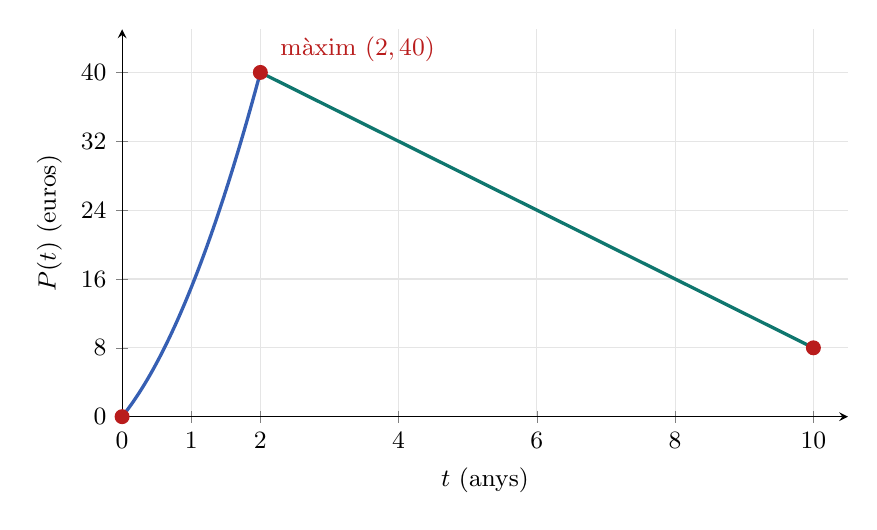
\begin{tikzpicture}
\begin{axis}[
  width=10.8cm,height=6.5cm,axis lines=left,
  xmin=0,xmax=10.5,ymin=0,ymax=45,
  xlabel={$t$ (anys)},ylabel={$P(t)$ (euros)},
  xtick={0,1,2,4,6,8,10},ytick={0,8,16,24,32,40},
  grid=major,grid style={black!10},tick label style={font=\small},label style={font=\small},clip=false]
  \addplot[tramU,very thick,domain=0:2,samples=100]{5*(x+1)^2-5};
  \addplot[tramDos,very thick,domain=2:10]{-4*x+48};
  \addplot[only marks,mark=*,mark size=2.5pt,punt] coordinates {(0,0) (2,40) (10,8)};
  \node[anchor=south west,font=\small,text=punt] at (axis cs:2.15,40.1) {màxim $(2,40)$};
\end{axis}
\end{tikzpicture}
\end{document}
